\documentclass{sig-alternate}
\usepackage{amsmath,epsfig}
\usepackage[caption=false]{subfig}
\usepackage{epstopdf}

\pagestyle{empty}
\begin{document}

%%

\title{
Selective Removal of Extraneous Photographs
}

\numberofauthors{4}
%\name{Anonymous submission}
\author{
\alignauthor
K. Armin Samii\\
       \email{ksamii@ucsc.edu}
% 2nd. author
\alignauthor
Uliana Popov\\
       \email{uliana@soe.ucsc.edu}
% 3rd. author
\and 
\alignauthor
Allison Carlisle\\
       \email{acarlisl@ucsc.edu}
% 4th. author
\alignauthor
James Davis\\
       \email{davis@soe.ucsc.edu}
}
%\name{K. Armin Samii, Allison Carlisle, Uliana Popov, James Davis}
%\address{[ksamii,acarlisl]@ucsc.edu,[uliana,davis]@soe.ucsc.edu}

\maketitle	
\begin{abstract}
In this paper, we propose a method for selecting the most representative high-quality images from a set of user photographs. To avoid redundancy arising from many similar images, we find all sets of near-duplicates. We then rank images based on three technical qualities: exposure, blur, and contrast. Finally, we provide an ordering of the images which accounts for both quality and uniqueness. Our goal is not to rank images based on subjective aesthetic qualities, but instead to help a photographer filter out technically flawed photographs and focus on objectively high quality shots.
\end{abstract}

\category{K.8.3}{Computing Milieux}{Personal Computing}

\terms{Management}

\keywords{image processing, quality screening, exposure, meta data, color content}

\section{Introduction}


\label{sec:intro}
%With the ease of digital cameras, both amateur and professional photographers take more pictures than they will need. An organized user will delete excess photos and keep the most important ones. We need something like: The digitalization has led to an ever increasing size of personal photo collections. Today, consumers often take hundreds or even thousands of pictures of an event.

The ease of using digital cameras allows for a large number of photographs to be taken at any given event. This increase in photograph quantity can lead to many unwanted low-quality photographs that need to be filtered by the user, which can be time-consuming and repetitive.

To automate this process, an aesthetics ranking technique could be implemented to find the appeal each image has, but this method would discard many images with potential to be fixed through retouching.

%So, a technical quality ranking technique can implemented, and the best images would be kept and the worst discarded. This method solves the previous problem, but does not take into account the redundancy of similar images, and the user would be left with a set which does not span their entire photo set.

Implementing a technical quality ranking technique will keep the photographs suited for retouching, but does not take into account redundancy of similar images, and the user would be left with a set which either includes many duplicates or does not span the entire event.

%To fix this, a similar image detector could be implemented giving the user the best image from every subset of similar images. This is still not ideal because it would leave the user with too many low-quality photographs that, although unique in the set, are not worth keeping.

We thus propose a technique which ranks images based on their technical qualities with a bias for unique images.%, but without forcing uniqueness by selecting the best from each set.

To focus our research and determine which image qualities are relevant to technical image quality, we assume three general steps a photographer takes between shooting and using a picture, which we call the Photographer's Process:
\begin{enumerate}
\item Remove: Sort through the imported images and remove the ones least suited for retouching.
\item Retouch: Modify the raw files just selected to stylize and enhance them.
\item Retrieve: Select the retouched images most suitable to a given task.
\end{enumerate}

This work focuses on the removal stage and contains both quality assessment and similarity ranking. We implement technical quality assessment using three modules: blur detection, exposure, and contrast. The blur detection uses three measures: the gradient magnitude of edges, the similarity to a predicted out-of-focus image, and the probability of a linear point-spread function existing. Exposure is measured by finding the balance in brightness throughout the image, both locally and globally. Contrast is measured based on the local changes in brightness throughout an image. We implement similarity ranking using global color similarity, foreground color similarity, and timestamps.  These modules are combined to obtain a reordering of the set representing how suited they are for removal (the "Importance Order"). A user study and tests with publicly available data has shown 89\% accuracy in our absolute ranking of photographs. The similarity ranking was evaluated separately and found to have 81\% accuracy. Fig. \ref{fig:Examples} shows our accuracy in finding the subject and rating quality.

\begin{figure*}
  \centering
    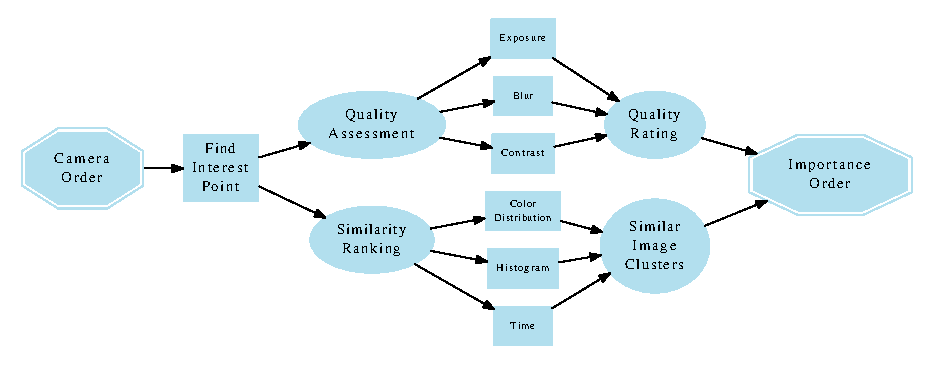
\epsfig{file=figures/flowchart.eps,width=16cm}
  \caption{Interest points are used to find the foreground subject. Blur, contrast, and exposure assessment algorithms are used to calculate an image's quality rating. Images are clustered into groups of similar images based on their histograms, color distribution, and timestamps. A reordering of the input results, allowing the user to remove images at the end of this ordering.}
  \label{flowchart}
\end{figure*}

\section{Related Work}

Previous works have classified images as professional vs. amateur with high accuracy\cite{1640788}\cite{springerlink:10.1007/11744078_23}\cite{springerlink:10.1007/978-3-540-88690-7_29}, which is useful for search engines' retrieval of high quality images. Others have focused on personalized \emph{aesthetic} rankings of photographs\cite {Sun:2009:PAB:1631272.1631351}\cite {Yeh:2010:PPR:1873951.1873963}. All of these works focus on finalized images, while we focus on images that are still raw and may be retouched afterwards.

Event classification has been explored in order to choose the best images from an entire event\cite{1223566}\cite{4444209}, while we choose the best images from each scene within each event: images with the same subject content rather than the same event context.

Kormann, Dunker, and Paduschek\cite{springerlink:10.1007/978-3-642-10543-2_23} describe a method of automatically rating and ranking images based on image content and time-metadata, but do not report numerical results, only that their results are better than random. 


\section{Quantifying Image Quality}

To find the Importance Order of the user's photographs, we use both quality assessment and similarity clustering. Quality is determined by the rankings of the blur, exposure, and contrast modules. Similarity of images is determined by matching the color content and timestamp of every pair of images. Both modules make use of a foreground region detection module based on interest points. We combine these measures to get the final ordering (Fig. \ref{flowchart}).

The quality modules (blur, exposure, and contrast assessment) provide a ranking between zero and nine, with larger numbers indicating higher quality. Because an image which is flawed in any of the three factors would be considered poor, we take the weighted sum-of-squares to penalize low scores more than we reward high scores. We assign weights to each module as follows: blur 50\%, exposure 40\%, and contrast 10\%.

\subsection{Foreground detection}\label{ContentRecognition}
Several modules make use of foreground detection. We use a Harris corner detector\cite{Harris} (utilizing NASA's Vision Workbench\cite{vision-workbench}) to obtain interest points for each image. To extract a bounding box from these points, the most dense rectangle is calculated by maximizing the ratio of interest points to rectangle area. We assume this to be the primary foreground subject.

\subsection{Exposure}

Exposure is a measure of how appropriate the lighting is in a given image. While easily measured in-camera using a light meter, we must evaluate the lighting condition based on pixel intensity.

To assess an image's exposure quality, we use both global and local calculations to compare the average grayscale value of the region to middle gray (halfway between black and white on a lightness scale)\cite{ppr:1815}.

The global method ranks an image highly when the average grayscale value is near middle gray. The local method divides the image into 20x20 grid. Images are ranked highly when the bright and dark grid cells average near middle gray, with no cells being extremely light or dark. We also penalize an image if there is not enough variation between grid cells. These two measures are averaged to provide a final ranking.

\subsection{Blur Detection}
There are three measures used to assess the amount of blur: edge width, global point-spread, and a comparison against a computed blurry image.

The first two rely on an edge-detection algorithm which is done in three steps. First, we calculate the differences between a pixel's luminosity and the image's average luminosity. Large differences are considered edge pixels. Mislabeled edge pixels are then removed by ensuring each one is connected to another edge pixel. Finally, edges are spaced out by ensuring there is a large radius of non-edge pixels around each set of edge pixels; if there is not, the edge pixel with the largest difference value from the first step is kept. % XX FIGURE?

The first measure finds the width of each edge by finding a "line of maximum contrast" from the brightest to darkest pixel around each edge pixel. Sharper edges will have shorter line lengths.

The second measure looks at the orientation of the lines of maximum contrast. If there are significantly more lines oriented in a single direction than the average, we assume the point-spread to be in that direction. %XX def. needs a figure

Finally, if the previous two measures are inconclusive, we compute a predicted blurred model of the foreground using a Gaussian blur filter on the image. The closer an image is to this model, the blurrier it is.

These three values are combined to determine the amount of blur. Only one needs to have high confidence for the final result. The results are averaged if none have high confidence.%, and it is especially accurate when comparing two similar images. % XX add result here, keep sentence?


\subsection{Contrast}

Contrast is the difference in visual properties that makes an object distinguishable from other objects and the background.
We use luminance contrast and
Root Mean Square (RMS) algorithm, which does not depend on the spatial frequency content or the spatial distribution of contrast in the image. It is defined as the standard deviation of the pixel intensities\cite{ppr:1982}.

\section{Similar-Image Clustering}
To find similar images we use three measures: time nearness, histogram similarity, and color distribution.

\subsection{Timestamp}
First, we use the timestamp to obtain a time similarity index between all pairs of images. Prior work focused on finding large timestamp gaps\cite{1292402}. We want to allow nonconsecutive images to be grouped together, so we have derived a formula which finds temporal closeness between every pair of images. We find the similarity \(S_{i,j}\) between two images \(i\) and \(j\) on a 0-9 scale:
\begin{eqnarray}
S_{i,j}=\frac{G_{i,j}}{A_{i,j}}
\end{eqnarray}
Where \(A_{i,j}\) is the average gap of the 8 images directly before \(i\) and after \(j\), and  \(G_{i,j}\) is the log of the time gap between the two images taken at time \(T_i\) and \(T_j\):
\begin{eqnarray}
G_{i,j}=\log(|T_i-T_j|)
\end{eqnarray}
The calculated similarity index \(S_{i,j}\) is used to weight the results of the next two steps.


\subsection{Histogram Similarity}
Directly comparing histograms will produce many false positives due to similar-colored images with different color distribution and content, and many false negatives due to changes in exposure affecting the histograms. Our method is robust against both of these.

The image is first divided into a 2x2 grid, with four pairs of values describing each grid cell: red, green, blue, and grayscale histograms, paired with the median color for each histogram. The grid protects against false positives. We then divide each histogram into 20 bins, each containing 5\% of the range of values, plus 2\% of the values in adjacent bins, which provides resistance against minor exposure changes. So, for example, the second bin will contain all pixels between 3\% and 12\%.

When comparing the histograms of two images, the bins are scaled so that all channels have the same median value. This provides resilience against larger exposure changes. A similarity ranking for each histogram is derived from the differences in the size of each scaled bin. Finally, each grid cell is weighted by the amount of the foreground that it contains. The result is the grid-weighted average of differences between each bin, with smaller differences indicating higher similarity:
\begin{eqnarray}
\mathrm{Difference_{I,J}}=\displaystyle\sum\limits_{g=1}^4W_g\sum\limits_{c=1}^4\sum\limits_{b=1}^{20} |I_{b,c} - J_{b,c}|
\end{eqnarray}
Where \(g\) is the grid cell, \(W_g\) is the weight of the cell based on foreground overlap, \(c\) is the channel, \(b\) is the bin, and \(|I_{b,c}-J_{b,c}|\) is the difference between the number of pixels in bin \(b\), channel \(c\) for images \(I\) and \(J\).

\subsection{Foreground Color Distribution}
We degrade an image to remove features from the foreground while maintaining general color and shape information by applying a strong Gaussian blur filter to the foreground. When comparing two images, a smaller pixel-by-pixel difference indicates higher similarity. Because only the foreground is used, this method is robust against composition changes and subject movement between photographs.

\subsection{Clustering}
Clusters are then formed using a Quality-Threshold algorithm. We first put each image into its own group, then iteratively merge the two most similar groups until a minimum similarity threshold is reached. In this way, groups votes for other similar groups, rather than single image voting for other images, resulting in a noise-resistant clustering. This method successfully groups panoramic sets of images together, even when the first image's histogram does not match the last image's. % Add panorama image?

To determine the Importance Order, we iteratively choose the image with the highest rank, then penalize every other image in the same set.

\section{Results}

\begin{figure*}[t!]
\centering
\subfloat[Unsorted]
{
	\fbox{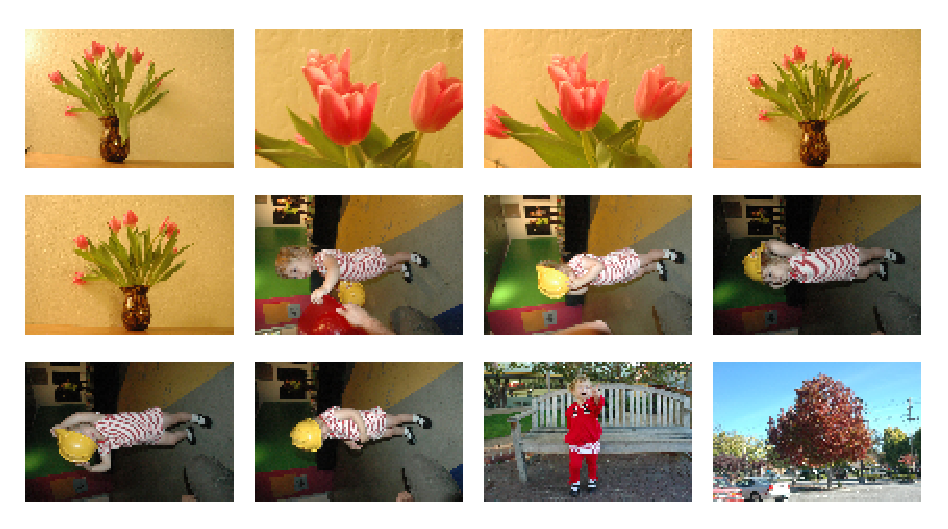
\epsfig{file=figures/result_unsorted.eps,width=8.5cm}}
	\label{resultunsorted}
}
\subfloat[Sorted]{
	\fbox{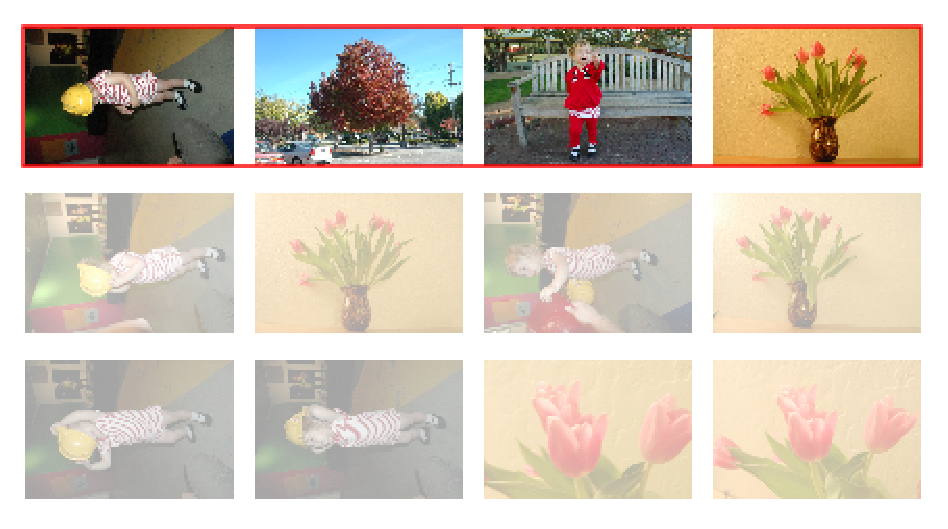
\epsfig{file=figures/result_sorted.eps,width=8.5cm}}
	\label{resultsorted}
}
\caption{\subref{resultunsorted} shows four sets of similar photographs provided by the user. \subref{resultsorted} shows the reordered set. We asked 10 Turk users to rank each image and we correctly chose the top image from each set.}
\label{fig:ResultSorting}
\end{figure*}

\begin{figure*}[t!]
\centering
\subfloat[Blurry]
{
	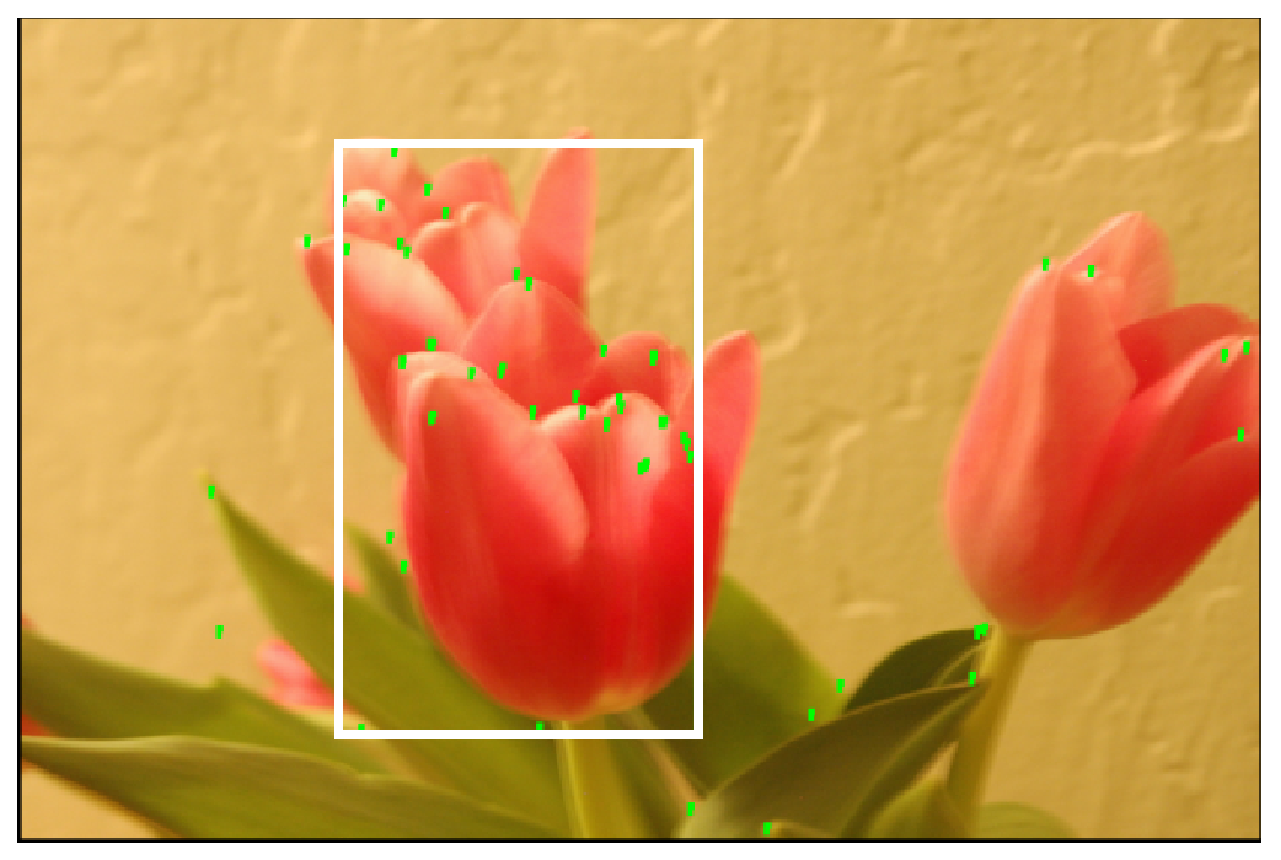
\epsfig{file=figures/example_blur.eps,width=5cm}
	\label{example_blur}
}
\subfloat[Overexposed]{
	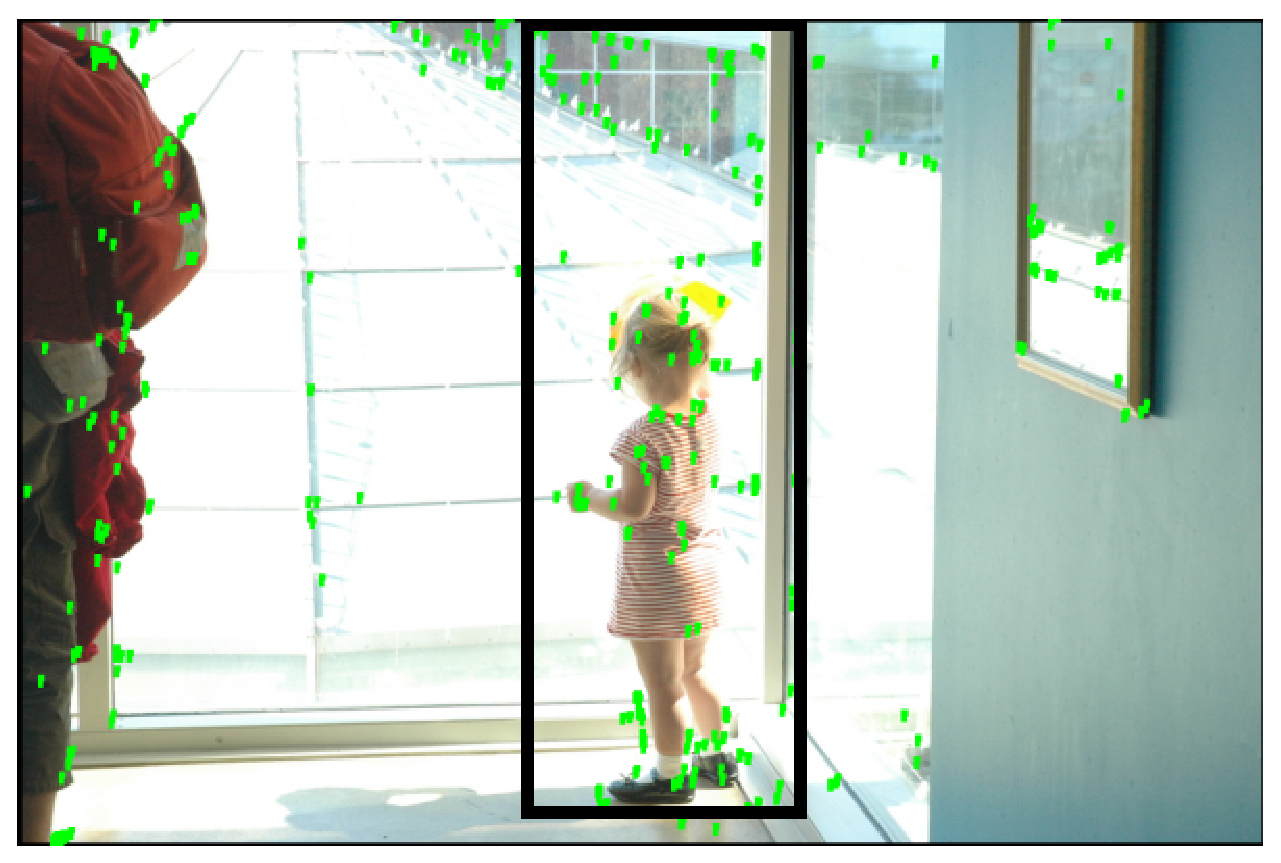
\epsfig{file=figures/example_expose.eps,width=5cm}
	\label{example_expose}
}
\subfloat[High quality]{
	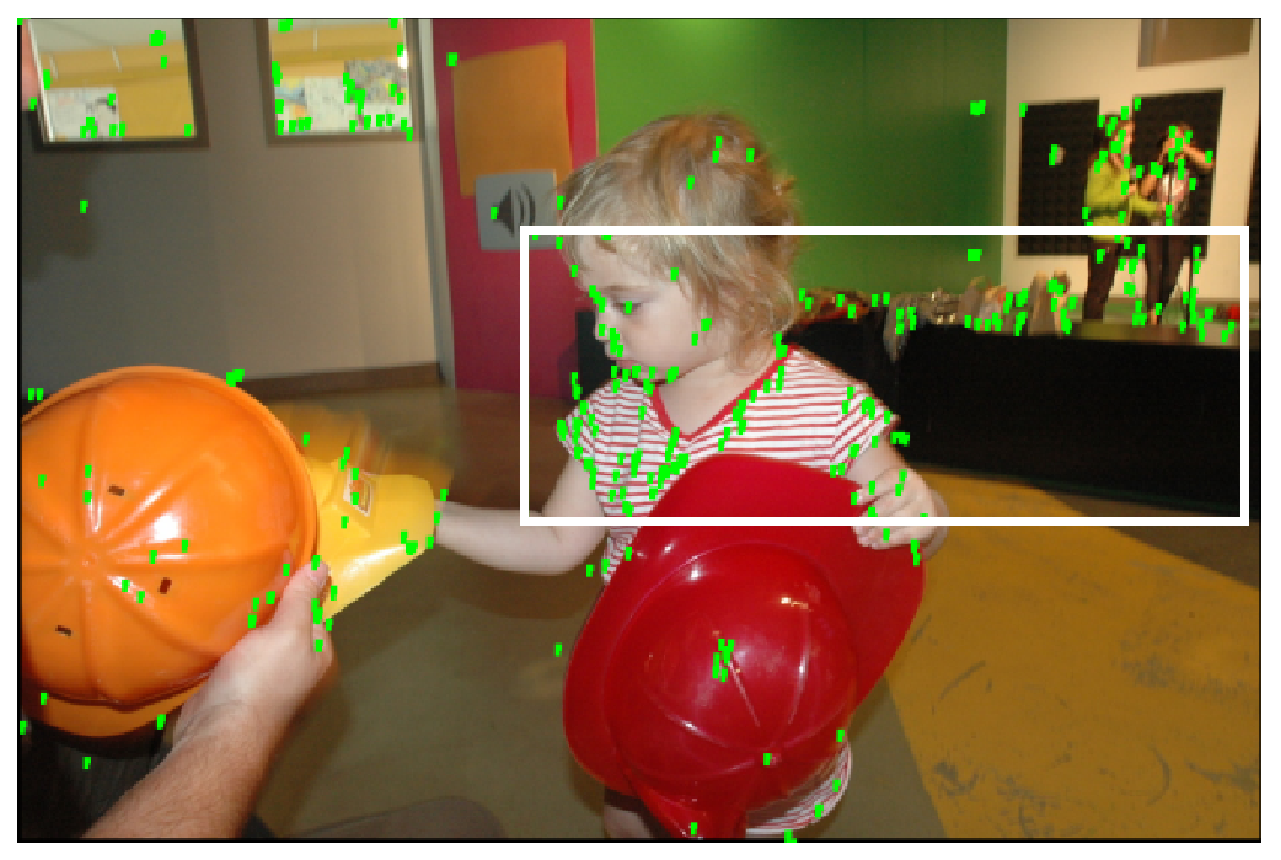
\epsfig{file=figures/example_good.eps,width=5cm}
	\label{example_good}
}
\caption{Examples of \subref{example_blur}\subref{example_expose} low quality and \subref{example_good} high-quality images, as determined by our modules. The dots are interest points found; the rectangle is the bounding box considered to be the subject.}
\label{fig:Examples}
\end{figure*}

We asked Amazon Mechanical Turk users to group together photographs within four sets of twenty images based on their own personal measure of "similarity." Our similarity index for each pair of images agrees with Turk users' decisions of whether a given pair of images is in the same group with 81\% accuracy.

We also assessed blur and exposure individually using a binary classification. First, we use our own data to confirm an image is low quality. We gathered 70 out-of-focus images uploaded by Turk users and correctly classified 62 of them as blurry (89\%). We then gathered 86 poorly exposed images (as determined by the in-camera light meter) and correctly classified 79 of them as having poor exposure (92\%).

To assess technically high quality images, we use INRIA's publicly available "Original Image" 157-image dataset\cite{JDS08}.  We correctly classified 139 as not blurry (89\%) and 135 as well-exposed (86\%). Averaging the four results gives 89\% accuracy overall.

Fig. \ref{fig:ResultSorting} shows an example of a user's input images being resorted by quality and uniqueness. The top four images in Fig. \ref{resultsorted} represent the highest quality images in each similar-image set. The nontrivial case of zoomed-in flowers was recognized as the same foreground subject. The top images are consistent with Turk users' votes.


\section{Conclusion and Future Work}
We propose a method of applying current research to automate another step of the Photographer's Process. By focusing on obtaining an ordering which is representative of all photographs taken, we obtain a diverse set of high quality images similar to what a user would have chosen manually. We derive a novel algorithm for analyzing exposure quality. We improve upon previous algorithms which find temporal gaps between images to obtain a metric for temporal nearness. The final Importance Order depends on both the quality ranking and the number of similar images which have appeared earlier in the ordering.

Our work focuses on a small portion of the Photographer's Process. In the future, we would like to see the three steps combined to automate the entire Process with minimal human input. This would facilitate a photographer's creativity by allowing more time spent on pure aesthetics and leaving technical details to the computer.

{
 \bibliographystyle{IEEEbib}
 \bibliography{bibliography}
}
\end{document}
